\graphicspath{ {fcu/} }

\section{Fan Coil Unit}

\subsection{Test Model}
The test model is developed based on the model of the FCU controller in VDMRT. Basically, it is a PID controller.

\subsubsection{Inputs and Outputs}
The SystemUdnerTest receives the following inputs (stimuli) from the TestEnvironment:
\begin{itemize}
    \item $RAT$: set point of room air temperature 
    \item $RATSP$: current room air temperature 
\end{itemize}

The SystemUdnerTest provides the following observable outputs to the TestEnvironment:
\begin{itemize}
    \item $fanSpeed$: fan speed  
    \item $valveOpen$: valve open state 
\end{itemize}

\subsubsection{Constant Variables and Local Variables}
Several constant variables below are defined. The access model property of all these variables is defined as \B{Read}.  
\begin{itemize}
	\item $K$: proportional gain
	\item $N$: derivative gain limitation
	\item $Td$: derivative time constant 
	\item $Ti$: integral time constant 
	\item $b$: proportional setpoint weighting parameter
	\item $c$: derivative setpoint weighting parameter 
    \item $sampletime$: sample time 
\end{itemize}

Other local variables are used to store intermediate results. However their access model property is set to \B{Read/Write}.

\begin{figure}[htb!]
    \centering
    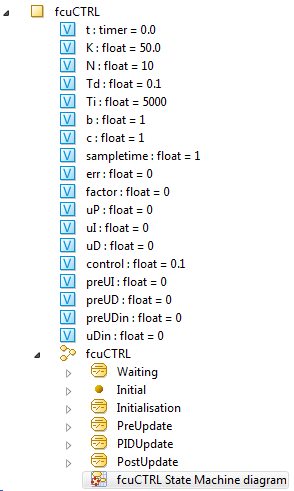
\includegraphics[width=0.4\textwidth]{fcu_sut_vars}
    \caption{Variables of LFR Controller}
    \label{fig:fcu-var}
\end{figure}


\subsubsection{State Machine Diagram}
When the state machine is residing in the \verb+Waiting+ state, it moves to processing states which are consisted of three states:
\begin{itemize}
    \item \verb+PreUpdate+: calculate numbers of local variables ($factor$, $err$, and $uDin$), that will be used in the next state, according to current inputs.
    \item \verb+PIDUpdate+: the transition of \verb+PreUpdate+ to this depends on the value of $RATSP$. If it is larger than 1, $uI$ will be updated. Otherwise, $uI$ is equal to 0. This is designed for anti integral windup.
    \item \verb+PostUpdate+: update $preUDin$, $preUI$ and $preUD$ that are used for sequential updates. 
\end{itemize}
Finally, the transition from \verb+PostUpdate+ to \verb+Waiting+ calculates (based on updated $uP$, $uI$ and $uD$) and outputs $fanSpeed$ and $valveOpen$ to its environment.

\begin{figure}[htb!]
    \centering
    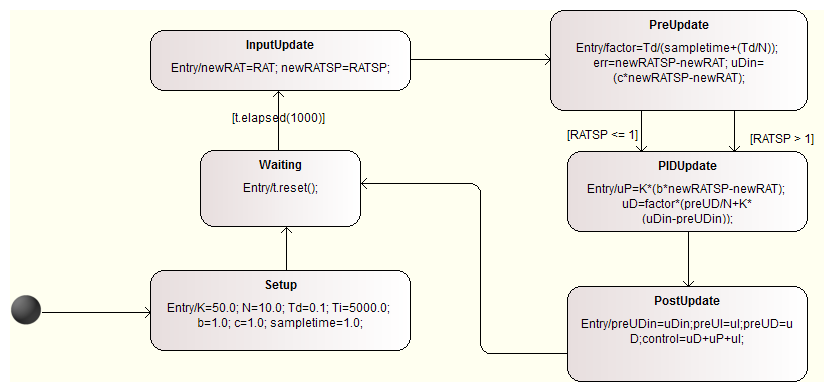
\includegraphics[width=1.0\textwidth]{fcu_sut_sm}
    \caption{State Machine Diagram of SUT}
    \label{fig:fcu-sut-sm}
\end{figure}

It is worth noting that
\begin{itemize}
    \item additional state \verb+Setup+ is used to set up all constants,
\end{itemize}

\subsection{A Manual Implementation of SUT in C}

The source code is listed as follows.

\lstset{language=C,
    basicstyle=\footnotesize\ttfamily,
    keywordstyle=\color{blue}\ttfamily,
    stringstyle=\color{red}\ttfamily,
    commentstyle=\color{green}\ttfamily,
    morecomment=[l][\color{magenta}]{\#},
    tabsize=2
}

\begin{lstlisting}
#include <stdio.h>
#include <sys/time.h>
#include <sys/types.h>
#include "fcu_ctrl.h"

const float K = 50.0;
const float Td = 0.1;
const float N = 10;
const float Ti = 5000;
const float b = 1;
const float c = 1;
const float sampletime = 1;

float err = 0;
float factor = 0;
float uDin = 0;
float uP = 0;
float uD = 0;
float uI = 0;
float control = 0.1;
float MV = 0;
float totaluI = 0;
float preUI = 0;
float totaluDin = 0;
float preuDin = 0;

#define _ms( t ) ( (t) * 1000 )

VSTimer_t t;

void reset( VSTimer_t* timer)
{
	struct timeval now;
	ti_gettimeofday( &now, NULL );
	*timer = now.tv_sec * 1000000 + now.tv_usec;
}

BOOLEAN elapsed( VSTimer_t* timer, long usec )
{
	struct timeval now;
	long long usec_now;

	ti_gettimeofday( &now, NULL );
	usec_now = now.tv_sec * 1000000 + now.tv_usec;
	return ( ( usec_now - (*timer) ) >= usec );
}

/** Initialize SUT */
void sut_init()
{
	reset(&t);
}

/** Run SUT (one step) */
void sut_run(float RAT, float RATSP, 
    float* fanSpeed, float* valveSpeed)
{
	err = RATSP - RAT;
	factor = Td/(sampletime + (Td/N));
	uP = K*(b*RATSP - RAT);

	if (RATSP > 1)
	uI = preUI + sampletime * (K * err/Ti);
	else
	uI = 0;
	preUI = uI;

	uDin = c*RATSP-RAT;
	uD = factor * (uD/N + K *(uDin - preuDin));
	preuDin = uDin;

	control = uP + uI + uD;
	*fanSpeed = control;
	*valveSpeed = control;

	return;
}
\end{lstlisting}

\subsubsection{Build of the implementation and Setup of Execution context Test Procedure}
A python script \verb+build-sut.py+ is used to build the SUT implementation and create the test procedure SUT under \verb+RTT_TestProcedures+. The main part is illustrated below.

\lstset{language={},
    basicstyle=\footnotesize\ttfamily,
    showstringspaces=false,
    tabsize=2
}
\begin{lstlisting}
print("## -- Building SUT -----------------------------")
try:
  print("## -- Wrapping SUT to FMU --------------------")
  os.chdir(os.path.join(context, "sut"))
  print("## Compiling sample SUT implementation in '{0}'".
    format(os.getcwd()))
  if 0 != os.system(" ".join([PROG_make,"all"])):
    raise NameError("Make Failed!")
  print("## Creating RTT_TestProcedures/SUT as wrapper to the 
    modelDescription.xml that fits to SUT".format(os.getcwd()))
  os.chdir(context)
  if not py(" ".join([PROG_wrap, "--model-description", 
      os.path.join(context, "RTT_TestProcedures", "Simulation", 
        "model", "modelDescription.xml"), 
      "RTT_TestProcedures/SUT"])):
    raise NameError("Wrapping of SUT failed")
  print("## -- Modifying test procedure...")
  append_to_file("""
// -- Added for SUT inclusion -----
CFLAGS  ; -I$(RTT_TESTCONTEXT)/sut
INCLUDE ; fcu_ctrl.h
LDPATH  ; -L$(RTT_TESTCONTEXT)/sut 
LDFLAGS ; -lfcu_ctrl
// --------------------------------
""", os.path.join(context, "RTT_TestProcedures", "SUT", 
    "conf", "swi.conf"))
define_sut_in_rts("""
@abstract machine sut()
{					   
	@INIT:{			   
		fprintf(stderr, "CALL SUT INIT\\n");
		sut_init();						   
	}									   
	@FINIT:{							   
		//
	}
	@PROCESS:{
		float RATSP;
		float RAT;
		float valveOpen;
		float fanSpeed;

		fprintf(stderr, "STARTING SUT PROCESS\\n");

		while(@rttIsRunning){
			/* Map FMU input variables to SUT: X = rttIOPre->X */
			RATSP = rttIOPre->RATSP;
			RAT = rttIOPre->RAT;

			sut_run(RAT, RATSP, &fanSpeed, &valveOpen);

			/* Map SUT output to FMU output: rttIOPost->X = X */
			rttIOPost->fanSpeed = fanSpeed;
			rttIOPost->valveOpen = valveOpen;

			@rttWaitSilent(1 _ms);
		}
	}
}
int ti_gettimeofday(struct timeval *tv, struct timezone *tz){
	tv->tv_sec	= @t / 1000;		  
	tv->tv_usec = (@t % 1000) * 1000;
	return 0; 
}
""", os.path.join(context, "RTT_TestProcedures", 
  "SUT", "specs", "fmi2sut.rts"))
\end{lstlisting}

\subsubsection{Project Actions}
An action named \verb+sut_build+ is added in the test project to build the SUT implementation and SUT test procedure automatically. The definition of its command is
\begin{verbatim}
c:/python27/python.exe <PROJECT-LOCAL-PATH>/sut/build-sut.py
\end{verbatim}

\subsection{Test Automation}

Not all test cases for BCS and TR are passed when running against simulation or SUT when latency of outputs is set to either 100ms or 10ms. Failures occur at time stamp 2101.
\lstset{language={},
    basicstyle=\scriptsize\ttfamily,
    showstringspaces=false,
    tabsize=2
}
\begin{lstlisting}
TM 00000002000 AM   2 N checker[fanSpeed]: state change: [indication ok] -> 
                        [new expected value] (value: 93.750495910644531)
TM 00000002000 AM   2 N checker[valveOpen]: state change: [indication ok] -> 
                        [new expected value] (value: 93.750495910644531)
TM 00000002101 AM   2 E FAIL (1) : TC-INTO-CPS-Demo-BCS-0006, TC-INTO-CPS-Demo-BCS-0002
                        @rttAssert expression in file rttSignalChecker.rts, line 701 evaluates to 0:
                        rttmbt_valueAcceptable(observed, expected, admissibleError, type, &deviation)
TM 00000002101 AM   2 N Checked signal: fanSpeed
TM 00000002101 AM   2 N observed value: 0, expected value: 93.750495910644531, 
                      admissible error: 9.9999999999999995e-008, deviation: 93.750495910644531
TM 00000002101 AM   2 N Failure description: latency elapsed for expected SUT output change.
TM 00000002101 AM   2 N checker[fanSpeed]: state change: [new expected value] -> [error detected]
TM 00000002101 AM   2 E FAIL (2) : TC-INTO-CPS-Demo-BCS-0006, TC-INTO-CPS-Demo-BCS-0002
                        @rttAssert expression in file rttSignalChecker.rts, line 701 evaluates to 0:
                        rttmbt_valueAcceptable(observed, expected, admissibleError, type, &deviation)
TM 00000002101 AM   2 N Checked signal: valveOpen
TM 00000002101 AM   2 N observed value: 0, expected value: 93.750495910644531, 
                        admissible error: 9.9999999999999995e-008, deviation: 93.750495910644531
TM 00000002101 AM   2 N Failure description: latency elapsed for expected SUT output change.
TM 00000002101 AM   2 N checker[valveOpen]: state change: [new expected value] -> [error detected]
\end{lstlisting}

However all are passed when the latency of outputs is set to 1000ms though there are two warnings. But the latency should be wrong.

\begin{lstlisting}
TM 00000003000 AM   2 W WARNING (1) : A new expected value 0 for signal fanSpeed did 
                        occur while still checking the last expected value 93.750495910644531
                        @rttCheck expression in file rttSignalChecker.rts, line 628 evaluates to 0:
                        current_state != rttmbt_new_expected
TM 00000003000 AM   2 P PASS: TC-INTO-CPS-Demo-BCS-0006, TC-INTO-CPS-Demo-BCS-0002
                        @rttAssert expression in file rttSignalChecker.rts, line 701 evaluates to 1:
                        rttmbt_valueAcceptable(observed, expected, admissibleError, type, &deviation)
TM 00000003000 AM   2 N Checked signal: fanSpeed
TM 00000003000 AM   2 N observed value: 0, expected value: 0, admissible error: 9.9999999999999995e-008, deviation: 0
TM 00000003000 AM   2 N checker[fanSpeed]: state change: [new expected value] -> [indication ok]
TM 00000003000 AM   2 W WARNING (2) : A new expected value 0 for signal valveOpen did 
                        occur while still checking the last expected value 93.750495910644531
                        @rttCheck expression in file rttSignalChecker.rts, line 628 evaluates to 0:
                        current_state != rttmbt_new_expected
TM 00000003000 AM   2 P PASS: TC-INTO-CPS-Demo-BCS-0006, TC-INTO-CPS-Demo-BCS-0002
                        @rttAssert expression in file rttSignalChecker.rts, line 701 evaluates to 1:
                        rttmbt_valueAcceptable(observed, expected, admissibleError, type, &deviation)
TM 00000003000 AM   2 N Checked signal: valveOpen
\end{lstlisting}

Some important points:
\begin{itemize}
    \item previously, do-action is used to initialise constants in the states \verb+Setup+. However, it seems that it has not executed. The operational semantics of do-actions is given in~\cite{VSI-mbt-man}: \I{if no state machine transition is enabled, the active simple state’s do-action and those of its ancestors are executed}. Eventually, since \verb+Setup+ is not a stable state, it will change to \verb+Waiting+ immediately and its do-action is not executed.
    \item it is necessary to change admissible errors of signal map, such as 0.0000001.
    \item TODO: find out the cause of failures for Simulation or SUT.
\end{itemize}

\subsection{Model Checking}
\begin{description}
    \item[P1] Constants will not be changed. 
\begin{verbatim}
Finally ([IMR.SystemUnderTest.fcuCTRL.fcuCTRL.Setup] and 
  Next (Globally ( [
    IMR.SystemUnderTest.fcuCTRL.K == 50.0 && 
    IMR.SystemUnderTest.fcuCTRL.N == 10.0 && 
    IMR.SystemUnderTest.fcuCTRL.Td == 0.1 && 
    IMR.SystemUnderTest.fcuCTRL.Ti == 5000 && 
    IMR.SystemUnderTest.fcuCTRL.b == 1 && 
    IMR.SystemUnderTest.fcuCTRL.c == 1 && 
    IMR.SystemUnderTest.fcuCTRL.sampletime == 1
])))
\end{verbatim}
    \item[P2] $fanSpeed$ of (RATSP=20, RAT=10) is larger than that of (RATSP=20, RAT=15)
    \item[P3] $RAT$ will approach $RATSP$  (how to simulate environment?)
\end{description}


\section{Fan Coil Unit (With Room and Wall)}
\subsection{Test Model}
The developed test model includes the FCU controller, the Room and Wall models. We use the Euler method to model continuous parts Wall and Room. 

\subsubsection{Inputs and Outputs}
The SystemUdnerTest receives the following inputs (stimuli) from the TestEnvironment:
\begin{itemize}
    \item $OAT$: outside air temperature 
    \item $RATSP$: room air temperature set point
\end{itemize}

The SystemUdnerTest provides the following observable outputs to the TestEnvironment:
\begin{itemize}
    \item $RAT\_out$: room air temperature 
\end{itemize}

\subsubsection{SystemUnderTest}
The SystemUnderTest consists of a FCU controller, a wall model and a room model.

The architecture diagram of SystemUnderTest is shown in Figure~\ref{fig:fcu_sut_sad}. 
\begin{figure}[htb!]
    \centering
	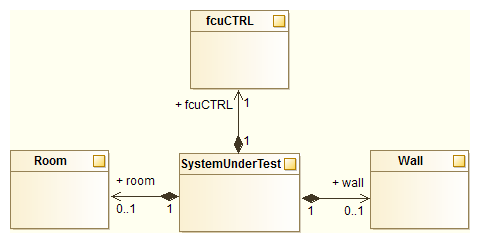
\includegraphics[width=0.8\textwidth]{roomwall/fcu_sut_sad}
    \caption{Architecture Diagram of SUT}
    \label{fig:fcu_sut_sad}
\end{figure}

\subsubsection{FCU Controller}
\paragraph{Inputs and Outputs}
The fcuCTRL receives the following inputs (stimuli):
\begin{itemize}
    \item $RAT\_out$: room air temperature from Room
    \item $RATSP$: room air temperature set point from TestEnvironment
\end{itemize}

The fcuCTRL provides the following outputs to the Room:
\begin{itemize}
    \item $fanSpeed$: fan speed 
    \item $valveOpen$: valve open state
\end{itemize}

The state machine diagram of fcuCTRL is illustrated in Figure~\ref{fig:fcu_sut_fcuctrl_sm}.
\begin{figure}[htb!]
    \centering
	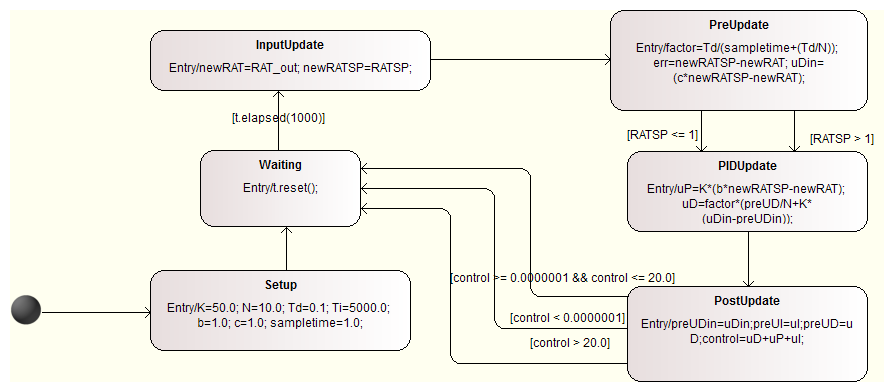
\includegraphics[width=1.0\textwidth]{roomwall/fcu_sut_fcuctrl_sm}
    \caption{State Machine Diagram of fcuCTRL}
    \label{fig:fcu_sut_fcuctrl_sm}
\end{figure}

\begin{itemize}
    \item \verb+Setup+ is used to initialize constant variables,
    \item After, the state machine resides in the \verb+Waiting+ state most of the time,
    \item After every one second, it starts to calculate PID parameters again,
        \begin{itemize}
            \item At first, update inputs $RAT$ and $RATSP$,
            \item Then calculate $uP$, $uD$, $uI$, and update other local variables for future use,
            \item Next calculate summation of $uP$, $uD$, and $uI$ to get $control$,
            \item Finally, limit $control$ and assign it to $fanSpeed$ and $valveSpeed$.
        \end{itemize}
\end{itemize}

\subsubsection{Wall}
\paragraph{Inputs and Outputs}
Wall receives the following inputs (stimuli):
\begin{itemize}
    \item $RAT\_out$: room air temperature from Room 
    \item $OAT$: outside air temperature from TestEnvironment 
\end{itemize}

Wall provides the following outputs to Room:
\begin{itemize}
	\item $Tisurf$: wall internal surface temperature
\end{itemize}

The state machine diagram of Wall is illustrated in Figure~\ref{fig:fcu_sut_wall_sm}.
\begin{figure}[htb!]
    \centering
	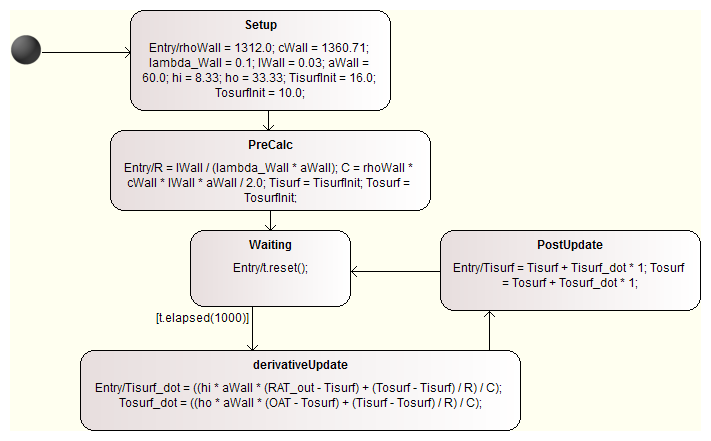
\includegraphics[width=1.0\textwidth]{roomwall/fcu_sut_wall_sm}
    \caption{State Machine Diagram of Wall}
    \label{fig:fcu_sut_wall_sm}
\end{figure}

\subsubsection{Room}
\paragraph{Inputs and Outputs}
Room receives the following inputs (stimuli):
\begin{itemize}
    \item $fanSpeed$: fan speed from fcuCTRL
    \item $valveOpen$: valve open state from fcuCTRL
	\item $Tisurf$: wall internal surface temperature from Wall
\end{itemize}

Room provides the following outputs to fcuCTRL and TestEnvironment:
\begin{itemize}
    \item $RAT\_out$: room air temperature
\end{itemize}

The state machine diagram of Room is illustrated in Figure~\ref{fig:fcu_sut_room_sm}.
\begin{figure}[htb!]
    \centering
	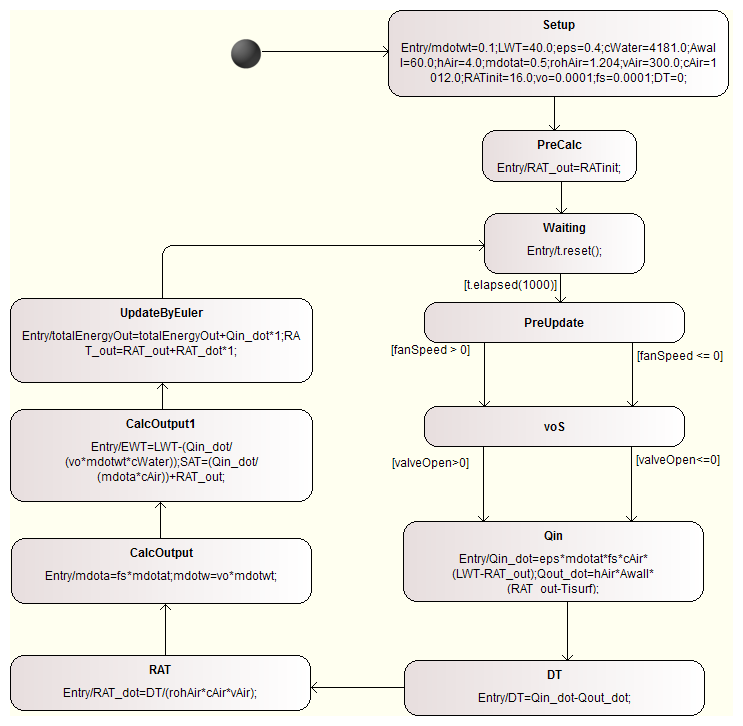
\includegraphics[width=1.0\textwidth]{roomwall/fcu_sut_room_sm}
    \caption{State Machine Diagram of Room}
    \label{fig:fcu_sut_room_sm}
\end{figure}

\subsection{Manual Implementations of SUT in C}
Two SUTs are implemented manually,
\begin{itemize}
    \item one standalone SUT to implement fcuCTRL, Room and Wall in C (correspond to SystemUnderTest in the test model),
    \item another SUT to implement fcuCTRL only in C, and then use the RoomHeating FMU from either 20-Sim or Modelica for Room and Wall.
\end{itemize}

\subsection{Test Automation}
\subsubsection{Test Input Sequence}
The inputs to FCU, $OAT$ and $RATSP$, is simulated through a state machine diagram in TestEnvironment. They are shown as $SUT\_OAT$ and $SUT\_RATSP$ in Figure~\ref{fig:fcu_co-sim-result}. $OAT$ changes slightly but $RATSP$ vibrates between 10 and 35 degrees.

\subsubsection{Test Run Configurations}
Three test configurations are provided for test automation with COE.
\begin{description}
    \item[SIM] TP against Simulation (Simulation is a SUT created from the test model), 
    \item[SUT] TP against the standalone SUT, 
    \item[SUT\_RoomWall] TP against the fcuCTRL SUT and RoomHeating FMU (therefore three FMUs).
\end{description}

Their test results are displayed in Figure~\ref{fig:fcu_co-sim-result}.
\begin{figure}[htb!]
    \centering
	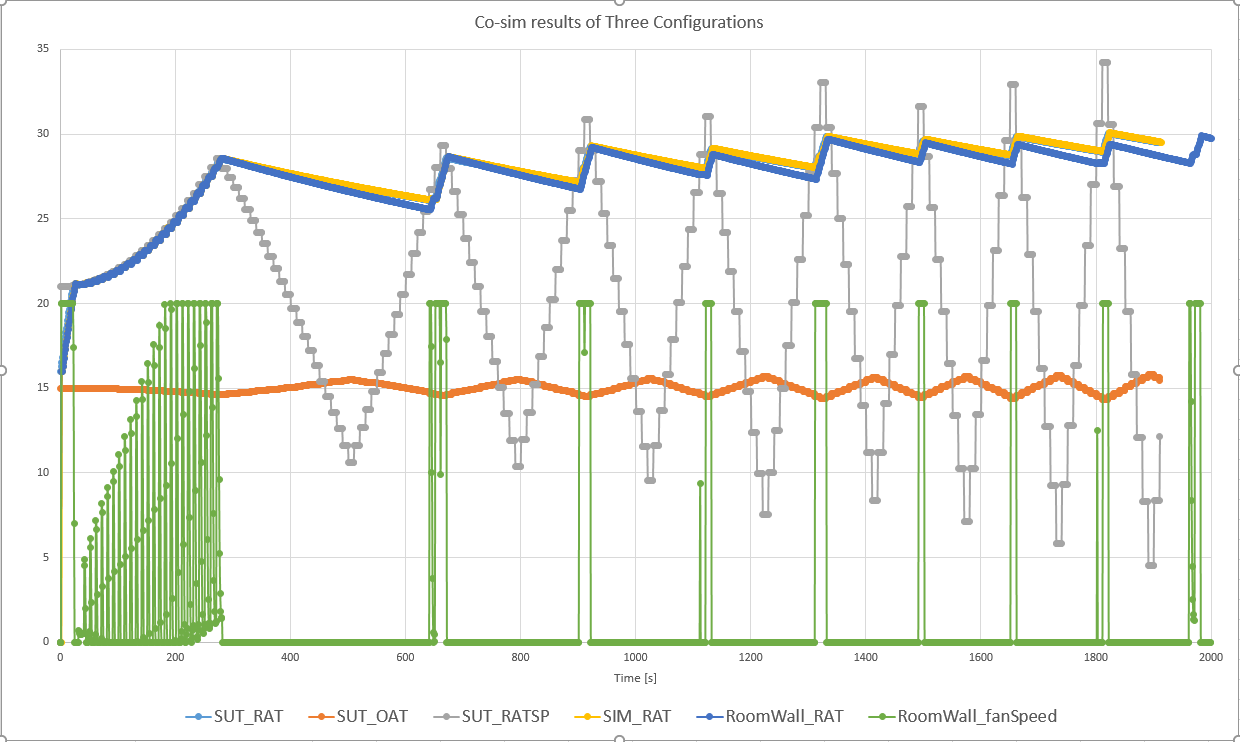
\includegraphics[width=1.0\textwidth]{test_results-20170621/fcu_co-sim-result}
    \caption{Test Results of Three Configurations}
    \label{fig:fcu_co-sim-result}
\end{figure}

From the diagram, we can see that
\begin{itemize}
    \item the change of set points will be reflected in the output $RAT$ though there are delays for the output to follow,
    \item the time to decrease temperature is longer than that to increase temperature,
    \item the fan speed is higher when desiring higher temperature, and is very low when wanting lower temperature,
    \item the output $RAT$ from \B{SUT} almost overlaps with that of \B{SIM} (because both of them uses the Euler method for Room and Wall), 
	\item the output $RAT$ from \B{SUT\_RoomWall} is slightly different from those of \B{SIM} and \B{SUT} (because the RoomHeating 20-Sim model uses the Runge Kutta 4 method).
        \begin{itemize}
            \item For \B{SUT\_RoomWall}, increase and decrease temperature faster than other two configurations.
        \end{itemize}
\end{itemize}

\subsection{Model Checking}
